\subsection{Aproximación cuasiestática}
\subsubsection{Dipolo eléctrico (caso estático)}

En electrodinámica clásica, se entiende como \textit{límite cuasiestático} el considerar a la partícula a estudiar mucho menor que la longitud de onda de la luz incidente. \cite{Cuasiest} En el caso de una elipsoide caracterizado por una función dieléctrica $\epsilon_p$, de semieje mayor $a$ que se encuentra inmerso en un medio caracterizado por una función dieléctrica $\epsilon_m$, estrictamente se puede definir el límite cuasiestático cuando el parámetro de tamaño $x=ka$ es mucho menor que la unidad \cite{Bohren}, donde $k=2\pi \sqrt{\epsilon_m}/\lambda$ representa el número de onda. Esta aproximación garantiza que el elipsoide esté sujeto a un campo eléctrico de la misma intensidad y dirección. \cite{Miguel}\\


En distancias mucho mayores que el tamaño de una partícula, es posible aproximar a esta como un \textit{dipolo eléctrico puntual}, por lo cual, es conveniente estudiar el potencial y campo eléctrico que produce.\\

Un dipolo físico consiste en dos cargas puntuales $q$ y $-q$ separadas a una distancia $d$ (ver Fig.\ref{dipolo_elec}), con momento dipolar $\Vec{p}=p\hat{e}_z$ donde $p=qd$. Si las cargas se encuentran embebidas en un medio homogéneo e infinito con función dieléctrica $\epsilon_m$, entonces el potencial $\phi$ del dipolo en un punto $P$ en $\Vec{r}$ es \cite{Bohren,Griffiths}
\begin{equation}
    \phi(\Vec{r})=\frac{q}{4\pi\epsilon_m}\left(\frac{1}{r_+}-\frac{1}{r_{-}}\right),    
\end{equation}
con,
\begin{equation*}
  \frac{1}{r_{\pm}}=\frac{1}{r}\left(1+\left(\frac{d}{2r}\right)^2\mp \frac{\Vec{r}\cdot\hat{e}_z}{r^2}d\right)^{-1/2}   \approx\frac{1}{r}\left(1\mp \frac{\Vec{r}\cdot\hat{e}_z}{r^2}d\right)^{-1/2}\approx\frac{1}{r}\left(1\pm \frac{\Vec{r}\cdot\hat{e}_z}{2r^2}d\right).  
\end{equation*}
donde el primer término se origina de considerar la ley de cosenos con $\cos\theta=\Vec{r}\cdot\hat{e}_z/r$,. La primera aproximación surge debido a que la región de interés es para $r\gg d$ de forma que el segundo término tiende a cero y la segunda aproximación se obtiene de la expansión binomial a primer orden de $(1\mp x)^n=1+nx$.
De esta forma,
\begin{equation}
    \frac{1}{r_+}-\frac{1}{r_{-}}\approx\frac{1}{r}\left(1+ \frac{\Vec{r}\cdot\hat{e}_z}{2r^2}d-1+ \frac{\Vec{r}\cdot\hat{e}_z}{2r^2}d\right)\approx\frac{1}{r}\left( \frac{\Vec{r}\cdot\hat{e}_z}{r^2}d\right)=\frac{\Vec{r}\cdot\hat{e}_z}{r^3}d.    
\end{equation}
Si $d$ se aproxima a cero de tal forma que $qd$ permanezca constante \cite{Bohren}, se obtiene el potencial para un dipolo puntual
\begin{equation}
\phi=\frac{p}{4\pi\epsilon_m}\left(\frac{\Vec{r}\cdot\hat{e}_z}{r^3}\right)=\frac{\Vec{p}\cdot\Vec{r}}{4\pi\epsilon_m r^3}=\frac{p\cos\theta}{4\pi\epsilon_m r^2}.
\label{pot_dipolo}
\end{equation}

\begin{figure}[h!]
	\centering
	\includegraphics[width=4.5cm]{../../Figuras/dipolo}
	\caption{Esquema de un dipolo físico. Se muestran dos cargas puntuales de carga $q$ y $-q$ separadas a una distancia $d$, así como un punto $P$ localizado en $\Vec{r}$. La distancia entre el punto P y las cargas $q$ y $-q$ está dada por $r_+$ y $r_{-}$, respectivamente. }
	\label{dipolo_elec}
\end{figure}

\subsubsection{Dipolo eléctrico (caso dinámico)}
Dado que el interés está en el caso en el que el campo incidente es una onda plana variando en el tiempo y en el espacio, se puede considerar un sistema de cargas y corrientes variando con el tiempo, hacer una expansión en series de Fourier de la dependencia del tiempo y manejar cada componente de Fourier por separado. De esta forma, no se pierde generalidad de considerar a los potenciales y campos de un sistema localizado de cargas y corrientes variando en el tiempo y que oscilan a la frecuencia $\omega$ del campo aplicado \cite{Jackson}
\begin{align}
    \rho(\Vec{r},t)&=\rho(\Vec{r})e^{-i\omega t},\nonumber\\
    \Vec{J}(\Vec{r},t)&=\Vec{J}(\Vec{r})e^{-i\omega t},
    \label{armonicf}
\end{align}
considerando que el significado físico lo posee la parte real y que las fuentes están consideradas localizadas en el espacio vacío. Por consiguiente, las Ecuaciones de Maxwell están dadas por
\begin{align}
	\nabla\cdot\Vec{E}&=0,\\
	\nabla\cdot\Vec{H}&=0,\\
	\nabla\times\Vec{E}&=i\omega\mu\Vec{H},\\
	\nabla\times\Vec{H}&=-i\omega\epsilon\Vec{E},
\end{align}
donde $\Vec{B}=\nabla\times\Vec{A}$, con $\Vec{A}$ el potencial vectorial y $ \Vec{H}=\Vec{B}/\mu_0$. Entonces,
\begin{equation}
	\Vec{H}=\frac{1}{\mu_0}\nabla\times\Vec{A}\hspace{0.5cm}\mbox{y}\hspace{0.5cm}    \Vec{E}=\frac{i}{\omega\epsilon}\nabla\times\Vec{H}.
\end{equation}

Si se consideran fuentes armónicas en el tiempo, como las mostradas en la Ec.(\ref{armonicf}), es posible determinar los campos electromagnéticos mediante el potencial vectorial, el cuál está dado por \cite{Jackson}
\begin{align*}
  \Vec{A}(\Vec{r},t)&=\frac{\mu_0}{4\pi}\int d^3r'\int dt'\frac{\Vec{J}(\Vec{r'},t')}{|\Vec{r}-\Vec{r'}|}\delta\left(t'-\left(t-\frac{|\Vec{r}-\Vec{r'}|}{c}\right)\right)\nonumber\\
  &=\frac{\mu_0}{4\pi}\int d^3r'\frac{\Vec{J}(\Vec{r'})e^{-i\omega \left(t-\frac{|\Vec{r}-\Vec{r'}|}{c}\right)}}{|\Vec{r}-\Vec{r'}|}=\frac{\mu_0}{4\pi}\int d^3r'\frac{\Vec{J}(\Vec{r'})e^{i\omega \frac{|\Vec{r}-\Vec{r'}|}{c}}}{|\Vec{r}-\Vec{r'}|}e^{-i\omega t},
\end{align*}
en donde se trabaja con la norma de Lorentz \cite{Griffiths} y en donde la función delta de Dirac está evaluada en el tiempo de retardo $t-|\Vec{r}-\Vec{r'}|/c$. Sea $k=\omega/c$ y omitiendo la dependencia temporal
\begin{equation}
    \Vec{A}(\Vec{r},t)=\frac{\mu_0}{4\pi}\int \Vec{J}(\Vec{r'})\frac{e^{ik|\Vec{r}-\Vec{r'}|}}{|\Vec{r}-\Vec{r'}|} d^3r'.
    \label{pot_vectorial}
\end{equation} 




Si las dimensiones de la fuente son del orden $d$ y la longitud de onda es $\lambda=2\pi c/\omega$, y $d\ll\lambda$, entonces hay tres regiones de interés: la región cercana (estática) en donde $d\ll r\ll\lambda$, la región intermedia en donde $d\ll r\sim \lambda$ y la región lejana (de radiación) donde $d\ll \lambda\ll r$.
En la región de campo cercano los campos, omitiendo la dependencia armónica, son como los campos estáticos con componentes radiales. En la región de campo lejano, los campos son transversales al vector de onda y decaen como $r^{-1}$. 
Para la región de campo cercano donde $r\ll\lambda$ (o $kr\ll 1$) la exponencial del potencial vectorial [Ec.\ref{pot_vectorial}] se aproxima a la unidad y con ello encontramos la expresión conocida de este \cite{Jackson}
\begin{equation*}
	\Vec{A}(\Vec{r},t)=\frac{\mu_0}{4\pi}\int \frac{\Vec{J}(\Vec{r'})}{|\Vec{r}-\Vec{r'}|} d^3r'.
\end{equation*} 


En la región de campo lejano ($kr\gg 1$) dado que la exponencial oscila rápidamente, determina el comportamiento del potencial vectorial. En esta región es suficiente aproximar

\begin{equation}
	|\Vec{r}-\Vec{r'}|\simeq r-\hat{e}_r\cdot\Vec{r'},    
\end{equation}
con $\hat{e}_r$ un vector unitario en la dirección de $\Vec{r}$. \footnote{Usando la ley de cosenos y haciendo una expansión binomial $
	|\Vec{r}-\Vec{r'}|=\sqrt{r^2+(r')^2-2rr'\cos\theta}=r\sqrt{1+\left(r'/r\right)^2-2\left((r'/r)\cos\theta\right)}\simeq r\left\{1-(\hat{e}_r\cdot\Vec{r'}/r)+1/2\left(r'/r\right)^2\right\}\simeq r-\hat{e}_r\cdot\Vec{r'}.$}
	
\begin{wrapfigure}{r}{6cm}%this figure will be at the right
	\centering
	\includegraphics[width=6cm]{../../Figuras/aprox}
	\caption{Vectores de posición $\Vec{r},\Vec{r'}$ del elemento de volumen dV y del punto P, respectivamente. Se muestra la distancia $|\Vec{r}-\Vec{r'}|$ entre estos últimos. }
\end{wrapfigure}
 Más aún, considerando la región de campo lejano, si sólo se consideran los términos que decaen como $r^{-1}$, el inverso de la distancia en la Ec.(\ref{pot_vectorial}) puede ser reemplazada por $r$. Entonces, el potencial vectorial es
\begin{equation*}
    \lim_{kr\rightarrow\infty}\Vec{A}(\Vec{r})=\frac{\mu_0}{4\pi}\frac{e^{ikr}}{r}\int \Vec{J}(\Vec{r'})e^{-ik\hat{e}_r\cdot\Vec{r'}}d^3r',    
\end{equation*}
que se puede reescribir al realizar la expansión en serie de potencias de la exponencial dentro de la integral de volumen, dando como resultado
\begin{equation*}
    \lim_{kr\rightarrow\infty}\Vec{A}(\Vec{r})=\frac{\mu_0}{4\pi}\frac{e^{ikr}}{r}\sum_n\frac{(-ik)^n}{n!}\int \Vec{J}(\Vec{r'})(\hat{e}_r\cdot\Vec{r'})^n d^3r'.    
\end{equation*}
Al considerar únicamente el primer término de la expansión como una primera aproxmación, se concluye que 
\begin{equation}
    \Vec{A}(\Vec{r})\approx\frac{\mu_0}{4\pi}\frac{e^{ikr}}{r}\int \Vec{J}(\Vec{r'}) d^3r',    
    \label{aprox_pot_vec}
\end{equation}
integrando por partes, \footnote{acá hay que hacer lo de la notación de tensores}
\begin{equation}
	\int\Vec{J}d^3r'=-\int \Vec{r'}(\nabla'\cdot\Vec{J})d^3r'=-i\omega\int \Vec{r'}\rho(\Vec{r'})d^3r',
	\label{Jrho}
\end{equation}
de donde se usa la ecuación de continuidad 
\begin{equation*}
    \nabla\cdot\Vec{J}=-\frac{\partial\rho}{\partial t}=i\omega\rho(\Vec{r}). 
\end{equation*}
Al sustituir la Ec.(\ref{Jrho}) en la Ec.(\ref{aprox_pot_vec}) y usando la definición del momento dipolar
\begin{equation*}
	\Vec{p}=\int \Vec{r'}\rho(\Vec{r'})d^3r',
\end{equation*}
se tiene que 
\begin{equation}
    \Vec{A}(\Vec{r})=-\frac{i\omega\mu_0}{4\pi}\frac{e^{ikr}}{r}\int \Vec{r'}\rho(\Vec{r'})d^3r'=-\frac{i\omega\mu_0}{4\pi}\frac{e^{ikr}}{r}\Vec{p} , 
    \label{A_dip}  
\end{equation}
con $\Vec{p}$ el momento dipolar eléctrico. Al calcular el campo H como el rotacional de $A/\mu$, y emplando la ley de Faraday-Lenz para determinar el campo eléctrico, se concluye que \footnote{Ver Apéndice A para el desarrollo de estas expresiones}
\begin{align}
	\Vec{E}&=\frac{i}{\omega\epsilon}\nabla\times\Vec{H}=\frac{1}{4\pi\epsilon_0}\left\{k^2(\hat{e}_r\times\Vec{p})\times\hat{e}_r\frac{e^{ikr}}{r}+[3\hat{e}_r(\hat{e}_r\cdot\Vec{p})-\Vec{p}]\left(\frac{1}{r^3}-\frac{ik}{r^2}\right)e^{ikr}\right\},\\
    \Vec{H}&=\frac{1}{\mu_0}\nabla\times\Vec{A}=\frac{ck^2}{4\pi}(\hat{e}_r\times\Vec{p})\frac{e^{ikr}}{r}\left(1-\frac{1}{ikr}\right).    
\end{align}
Obsérvese que el campo $\Vec{H}$ es transversal al vector radial para cualquier distancia, mientras el campo eléctrico tiene componentes paralelas y perpendiculares a $\hat{e}_r$.\\

\noindent En la zona de radiación cuando $kr\gg 1$ se tiene que \begin{align}
    \Vec{E}&=\sqrt{\frac{\mu_0}{\epsilon_0}}\Vec{H}\times\hat{e}_r=\frac{ck^2}{4\pi}(\hat{e}_r\times\Vec{p})\times\Vec{e}_r\frac{e^{ikr}}{r}=\frac{e^{ikr}}{-ikr}\frac{ik^3}{4\pi\epsilon_m}\hat{e}_r\times(\hat{e}_r\times\Vec{p}),\label{campoE}\\
    \Vec{H}&=\frac{ck^2}{4\pi}(\hat{e}_r\times\Vec{p})\frac{e^{ikr}}{r}.\label{campoH}  
\end{align}
Con base en la Ec. (\ref{A_dip}) al iluminar el sistema con una onda plana monocromática de frecuencia angular $\omega$, el dipolo inducido $p$ [Ec. (16)] y por tanto los campos electromagnéticos $\Vec{E}$ y $\Vec{H}$ [Ecs. (\ref{campoE}) y (\ref{campoH})] oscilarán a esa misma frecuencia. Por lo tanto, los campos electromagnéticos esparcidos $\Vec{E}_{s}$ y $\Vec{H}_{s}$, generados por el dipolo inducido, son
\begin{align}
    \Vec{E}_{s}&=\frac{e^{ikr}}{-ikr}\frac{ik^3}{4\pi\epsilon_m}\hat{e}_r\times(\hat{e}_r\times p) e^{i\omega t},\\
    \Vec{H}_{s}&=\frac{ck^2}{4\pi}(\hat{e}_r\times\Vec{p})\frac{e^{ikr}}{r}e^{i\omega t}.
\end{align}
 Sustituyendo el momento dipolar de un dipolo puntual $\Vec{p}=\epsilon_m \alpha E_0 e^{-i\omega t}\hat{e}_x$, se pueden reescribir a los campos esparcidos como
 \begin{align}
 	\Vec{E}_{s}&=\frac{e^{ikr}}{-ikr}\frac{ik^3}{4\pi\epsilon_m}\left(\epsilon_m \alpha E_0 \right)\hat{e}_r\times(\hat{e}_r\times \hat{e}_x)=\frac{e^{ik(r-z)}}{-ikr}\frac{ik^3}{4\pi}\left( \alpha E_0 e^{ikz}\right)\hat{e}_r\times(\hat{e}_r\times \hat{e}_x)=\frac{e^{ik(r-z)}}{-ikr}\Vec{X}E,
 	\label{E_scat}\\
 	\Vec{H}_{s}&=\frac{k}{\omega\mu}\hat{e}_r\times\Vec{E}_{s}.
 	\label{H_scat}
 \end{align}
donde $E=E_0 e^{ikz}$ y $\Vec{X}=\frac{ik^3}{4\pi}\alpha \hat{e}_r\times(\hat{e}_r\times \hat{e}_x)$ es
el vector de amplitud de esparcimiento y su polarización en la base de vectores esféricos es $\Vec{p}=\epsilon_m \alpha E_0 e^{-i\omega t}(\sin\theta\cos\phi\: \hat{e}_r+\cos\theta\cos\phi\: \hat{e}_{\theta}-\sin\phi \:\hat{e}_{\phi})$ \footnote{Es decir, $\hat{e}_r\times(\hat{e}_r\times \hat{e}_x)=-\cos\theta\cos\phi \hat{e}_{\theta}+\sin\phi \hat{e}_{\phi}$. }. \\

